\documentclass[11pt]{article}
\usepackage[T1]{fontenc}
\usepackage{lmodern}
\usepackage[margin=1in]{geometry}
\usepackage{amsmath,amssymb,amsthm,mathtools}
\usepackage{microtype}
\usepackage{enumitem}
\usepackage{needspace}
\usepackage{float}
\usepackage{xcolor}
\usepackage{tikz}
\usepackage[colorlinks=true,linkcolor=blue!55!black,citecolor=blue!55!black,urlcolor=blue!55!black]{hyperref}

\newtheorem{theorem}{Theorem}[section]
\newtheorem{lemma}[theorem]{Lemma}
\newtheorem{proposition}[theorem]{Proposition}
\newtheorem{corollary}[theorem]{Corollary}
\theoremstyle{definition}
\newtheorem{definition}[theorem]{Definition}
\theoremstyle{remark}
\newtheorem{remark}[theorem]{Remark}

\newcommand{\R}{\mathbb R}
\newcommand{\Z}{\mathbb Z}
\newcommand{\N}{\mathbb N}
\newcommand{\E}{\mathbb E}
\newcommand{\Prob}{\mathbb P}
\newcommand{\one}{\mathbf 1}
\newcommand{\cA}{\mathcal A}
\newcommand{\cS}{\mathcal S}
\newcommand{\cC}{\mathcal C}
\newcommand{\norm}[1]{\left\lVert #1\right\rVert}
\newcommand{\abs}[1]{\left\lvert #1\right\rvert}
\newcommand{\TV}{\operatorname{TV}}
\newcommand{\dist}{\operatorname{dist}}
\newcommand{\Span}{\operatorname{span}}
\newcommand{\supp}{\operatorname{supp}}
\DeclareMathOperator{\conv}{conv}

\newcommand{\papertitle}{Nontrivial Markov Type Forces Superreflexivity}
\author{OpenAI}
\hypersetup{
 pdftitle={\papertitle},
 pdfauthor={OpenAI},
 pdfsubject={A proof that nontrivial Markov type forces superreflexivity of real Banach spaces},
 pdfkeywords={Markov type, superreflexivity, Banach spaces, reversible Markov chains}
}

\begin{document}
\begin{center}
 {\Large\papertitle\par}
 \vspace{0.5\baselineskip}
 {OpenAI\par}
 {September 23, 2026\par}
\end{center}
\vspace{0.5\baselineskip}

\begin{abstract}
We prove that every real Banach space with Markov type $p>1$ is
superreflexive. Together with the known converse, this characterizes
superreflexivity by nontrivial Markov type. This answers Naor's question:
every real Banach space with nontrivial Markov type admits an equivalent
uniformly smooth norm.
\end{abstract}

\section{Introduction}

A finite Markov chain $(Z_t)_{t\geq0}$ on a set $S$, with transition
matrix $P$ and initial distribution $\pi$, is \emph{stationary and reversible}
if
\[
 \pi_iP_{ij}=\pi_jP_{ji}\qquad(i,j\in S).
\]
A normed space $X$ has \emph{Markov type $p>0$ with constant $0<K<\infty$} if, for
every such chain, every $f:S\to X$, and every integer $t\geq1$,
\begin{equation}\label{eq:markov-type}
 \E\norm{f(Z_t)-f(Z_0)}^p
 \leq K^p t\,\E\norm{f(Z_1)-f(Z_0)}^p.
\end{equation}
A Banach space is \emph{superreflexive} if it admits an equivalent
uniformly convex norm. Here a norm $|\cdot|$ is equivalent to $\|\cdot\|$
if $a\|x\|\leq|x|\leq b\|x\|$ for some $a,b>0$; it is uniformly convex
if, for every $\epsilon\in(0,2]$, there is $\delta>0$ such that
\[
 |x|,|y|\leq1,\quad |x-y|\geq\epsilon
 \quad\Longrightarrow\quad
 \left|\frac{x+y}{2}\right|\leq1-\delta.
\]

\begin{theorem}\label{thm:main}
Every real Banach space with Markov type $p$ for at least one $p>1$
is superreflexive.
\end{theorem}

\paragraph{Context and result.}
Ball introduced Markov type to study Lipschitz extension from metric
spaces \cite{Ball}. The inequality tests every finite reversible walk,
so it is a metric property even when the target is a Banach space.
Superreflexivity, by contrast, is defined through an equivalent norm;
its metric characterizations are central examples in the Ribe program,
which seeks metric descriptions of linear-geometric properties.
Bourgain characterized it by the distortion of finite complete binary trees
\cite{Bourgain}; finite diamonds provide another metric test
\cite{JohnsonSchechtman}. Lee, Naor, and Peres introduced Markov
convexity in their study of tree distortion \cite{LeeNaorPeres}.
Mendel and Naor later characterized superreflexivity through
\emph{Markov convexity}, an inequality comparing walks that share their
past and then evolve independently \cite{MendelNaor}.
Theorem~\ref{thm:main} identifies what ordinary
Markov type alone detects for Banach spaces.
Ordinary Rademacher type, which controls sums with independent random
signs, does not suffice for this conclusion: James constructed
nonreflexive spaces of Rademacher type $2$ \cite{JamesType2}.

Naor, Peres, Schramm, and Sheffield showed that uniform smoothness of
power type $p$ implies Markov type $p$ for $1<p\leq2$ \cite{NPSS}.
Pisier's power-type renorming theorem \cite{Pisier} therefore gives
nontrivial Markov type to every superreflexive space; Markov type is
invariant under equivalent norms. Naor asked whether a Banach space
could have nontrivial Markov type without an equivalent uniformly smooth
norm \cite[Question~4]{Naor}. Since equivalent uniformly smooth and
uniformly convex renormings exist for precisely the superreflexive
spaces \cite{Pisier}, Theorem~\ref{thm:main} answers this question
negatively and completes the characterization for real Banach spaces.

The classical structural input is the James--Enflo characterization:
\begin{equation}\label{eq:superreflexive-characterization}
 \begin{gathered}
 X\text{ admits an equivalent uniformly convex norm}\\
 \Longleftrightarrow\\
 \text{every Banach space finitely representable in }X
 \text{ is reflexive}.
 \end{gathered}
\end{equation}
Here $Y$ is \emph{finitely representable} in $X$ if, for every
finite-dimensional $E\subseteq Y$ and every $\eta>0$, there is an
injective linear $T:E\to X$ with
$\norm{T}\norm{T^{-1}}<1+\eta$.
We use \eqref{eq:superreflexive-characterization} in its standard form
\cite{James,Enflo}; the other background tools are Hahn--Banach and the
finite Ramsey theorem. The finite-dimensional form of Goldstine's theorem
needed below is included in the proof.

\paragraph{Proof strategy.}
We argue by contradiction. The James--Enflo characterization supplies
a nonreflexive space finitely representable in a nonsuperreflexive one.
From it we construct a spreading norm $N$ on
finite sequences for which summing consecutive entries is contractive.
This is a concrete version of the equal-sign-additive construction of
Brunel and Sucheston
\cite{BrunelSucheston1974,BrunelSucheston1975,BrunelSucheston}.
Equal-sign additivity means that merging adjacent coefficients of the
same sign preserves the norm.
The finite-representability formulation and related graph-embedding
applications appear in \cite{Ostrovskii,OstrovskiiRandrianantoanina}.
We include the precise version and
its finite-representability proof in Appendix~\ref{app:norm}.

For each time $n$, the central task is a finite reversible walk with
unit edge labels, changing sign under reversal, whose sum has norm at
least $n/24$ with probability at least $3/20$. Before normalization,
the labels are sums of signed differences of standard basis vectors
in finite coefficient sequences. Their prefix sums are signed indicators
of unions of intervals. A reduced word acting on the
line makes selected prefix sums of the total label alternate between
two levels separated by its reduced length. Consecutive summation converts
these oscillations into a lower bound proportional to the reduced length,
measured in units of the common one-step label norm. Finite Ramsey averaging supplies
increasing charts from a finite set of real points to coefficient indices,
with matching marginal laws, so this
ordered motion can occur along reversible transitions.
The transition letters are independent and uniform; their reduced length
is proportional to $n$ with a fixed positive probability.

An edge label need not be the difference of values assigned to its two
chart states; a marked transition may carry a nonzero label even when
the chart state does not change. A finite lattice lift records traversed
oriented edges as
integer coordinates. Its potential has exactly the required increments
away from the boundary, and rejected boundary moves keep the lifted
chain reversible. Section~\ref{sec:reduction} proves this transfer and
reduces Theorem~\ref{thm:main} to the finite-walk target.
Section~\ref{sec:finite-lemmas} constructs chart transport,
Section~\ref{sec:action} constructs the two prefix levels, and
Section~\ref{sec:walks} assembles the walk and proves its displacement.

\section{Reduction to a finite walk}\label{sec:reduction}

The reduction has three inputs. Lemma~\ref{lem:ordered-norm} supplies
an ordered norm from nonsuperreflexivity, Proposition~\ref{prop:walks}
constructs a walk in that norm, and Lemma~\ref{lem:edge-labels}
transfers the Markov type inequality to its odd edge labels.

\subsection{The ordered norm}

Write $c_{00}$ for the real sequences with finite support, and $b_i$ for
the $i$th coordinate vector. Finite coefficient arrays are identified with
elements of $c_{00}$ by appending zeros.
A norm $N$ on $c_{00}$ is \emph{spreading invariant} if
\begin{equation}\label{eq:spreading}
 N\left(\sum_{i=1}^m a_i b_i\right)
 =N\left(\sum_{i=1}^m a_i b_{k_i}\right)
 \qquad(k_1<\cdots<k_m).
\end{equation}
Thus inserting or removing zero entries does not change the norm.

\begin{lemma}\label{lem:ordered-norm}
If a real Banach space $X$ is not superreflexive, there is a norm $N$
on $c_{00}$ such that:
\begin{enumerate}[label=\textup{(\roman*)},leftmargin=*]
 \item $N$ is spreading invariant;
 \item merging two adjacent entries is contractive:
 \begin{equation}\label{eq:merge}
  N(a_1,\ldots,a_{i-1},a_i+a_{i+1},a_{i+2},\ldots,a_m)
  \leq N(a_1,\ldots,a_m);
 \end{equation}
 \item every initial coordinate span, equipped with $N$, admits
 linear embeddings into $X$ with distortion arbitrarily close to $1$.
\end{enumerate}
\end{lemma}

The construction is proved in Appendix~\ref{app:norm}.
Repeated adjacent merging shows that replacing every block of a partition
into consecutive intervals by its sum is contractive.
Spreading invariance will allow us to place coordinates by increasing
maps, while consecutive summation will convert differences of prefix
sums into a norm lower bound.

\subsection{The finite-walk target}

A \emph{finite marked chain} has a finite state set
$S$ and a finite set of oriented edges $\mathcal E$. An edge $e$ has
source $e^-$, target $e^+$, and reverse $e^*$, where star is an involution
and $(e^*)^-=e^+$, $(e^*)^+=e^-$. The probability of choosing $e$ from
its source is $q(e)$, with $\sum_{e:e^-=z}q(e)=1$ for every state $z$.
We require a probability distribution $\pi$ satisfying
\begin{equation}\label{eq:edge-balance}
 \pi(e^-)q(e)=\pi(e^+)q(e^*).
\end{equation}
The state chain is then stationary and reversible when started in $\pi$.

Marks allow several distinct edges between the same states.
A labeling $g$ is \emph{odd} if $g(e^*)=-g(e)$ for every edge.

\begin{proposition}[A finite walk with linear displacement]\label{prop:walks}
Let $N$ be a spreading invariant norm on $c_{00}$ for which merging
adjacent entries is contractive. For every integer $n\geq1$, there are
a finite stationary reversible marked chain and an odd labeling $g$
in a finite coordinate span such that
\[
 N(g(e))=1\qquad\text{for every edge }e,
\]
and, for the first $n$ edges $E_1,\ldots,E_n$ of the stationary chain,
\begin{equation}\label{eq:unit-walk}
 \Prob\left\{N\left(\sum_{i=1}^n g(E_i)\right)
                 \geq\frac n{24}\right\}\geq\frac3{20}.
\end{equation}
\end{proposition}

The construction occupies Sections~\ref{sec:finite-lemmas}--\ref{sec:walks}.
The chain and coordinate dimension may depend on $n$; the numerical
constants do not.

\subsection{Applying Markov type to edge labels}

The labels in Proposition~\ref{prop:walks} need not be differences of a
function on the chart states. A finite lattice lift will turn them into
such differences and allow Markov type to control their sums.

The Markov type inequality passes to normed spaces finitely representable
in its target, with the same constant. More precisely, only the span of
the finitely many values of $f$ needs to admit embeddings with distortion
arbitrarily close to $1$. After scaling such an embedding $T$, we have
\[
 \norm{x}\leq\norm{Tx}_X\leq(1+\eta)\norm{x},
\]
so applying \eqref{eq:markov-type} in $X$ gives its counterpart in the
original target with constant $(1+\eta)K$. Let $\eta\downarrow0$.

\begin{lemma}[Odd edge labels]\label{lem:edge-labels}
Suppose $V$ is a normed space of Markov type $p$ with constant $K$.
For a finite marked chain satisfying \eqref{eq:edge-balance}, let
$g:\mathcal E\to V$ satisfy $g(e^*)=-g(e)$.
If $E_1,\ldots,E_n$ are its first $n$ edges, with initial state distributed
as $\pi$, then
\begin{equation}\label{eq:odd-markov}
 \E\norm{\sum_{i=1}^n g(E_i)}^p
 \leq K^p n\,\E\norm{g(E_1)}^p.
\end{equation}
The same conclusion holds if the finite span of the labels is finitely
representable in a space of Markov type $p$ with constant $K$.
\end{lemma}

\begin{proof}
Choose one edge $e_j$ from each two-element star orbit, $1\leq j\leq r$,
and let $u_j$ be the coordinate vectors of $\Z^r$.
Give $e_j$ displacement $u_j$ and $e_j^*$ displacement $-u_j$.
A fixed point of star has label zero and is given displacement zero.
If $r=0$, there is nothing to prove.

For an integer $R>n$, put $Q_R=\{-R,\ldots,R\}^r$.
Lift the chain to $S\times Q_R$ by choosing an edge as before and making
the corresponding lattice move. If the move would leave $Q_R$, remain
at the same full state. Every accepted transition satisfies detailed
balance under $\pi\otimes\operatorname{Unif}(Q_R)$ by
\eqref{eq:edge-balance}; rejections add only self-loop probabilities.
This is a finite stationary reversible chain.

Define
\[
 \Phi(z,a)=\sum_{j=1}^r a_jg(e_j).
\]
On an accepted edge its increment is $g(e)$, and on a rejection its
increment is zero. The expected one-step cost is therefore at most
$\E\norm{g(E_1)}^p$.
If the initial lattice point lies in $Q_{R-n}$, every possible sequence
of $n$ edges is accepted. Couple the lifted walk to the original marked
walk by using the same proposed edges until the first rejection. On this
interior event the first $n$ edges agree, and the event is independent of
the original marked trajectory. Its probability is
\[
 \alpha_R=\left(\frac{2(R-n)+1}{2R+1}\right)^r\longrightarrow1.
\]
Consequently the expected $n$-step cost of the lifted potential is at
least $\alpha_R\E\norm{\sum_{i=1}^n g(E_i)}^p$.
Applying Markov type to $\Phi$ gives
\[
 \alpha_R\E\norm{\sum_{i=1}^n g(E_i)}^p
 \leq K^p n\,\E\norm{g(E_1)}^p.
\]
Let $R\to\infty$. The last assertion follows from finite-dimensional
transfer; enlarging the cube does not enlarge the span of the labels.
\end{proof}

\subsection{Proof of the main theorem}

\begin{proof}[Proof of Theorem~\ref{thm:main}]
Suppose that $X$ has Markov type $p>1$ with constant $K$ and is not
superreflexive. Lemma~\ref{lem:ordered-norm} supplies a spreading
invariant norm $N$ with contractive adjacent merging, whose finite
coordinate spans embed in $X$ with arbitrarily small distortion.
For each $n$, apply Proposition~\ref{prop:walks} to $N$.
Lemma~\ref{lem:edge-labels}, applied through the finite span of these
labels, gives
\begin{equation}\label{eq:contradiction}
 \frac3{20}\left(\frac n{24}\right)^p
 \leq\E N\left(\sum_{i=1}^n g(E_i)\right)^p
 \leq K^p n.
\end{equation}
Since $n$ is arbitrary and $K$ is fixed, this contradicts $p>1$.
\end{proof}

All chains used in this deduction are finite and start in their
reversible stationary distributions. Their sizes and the embeddings
into $X$ may depend on $n$; only $K$ must be uniform.
It remains to construct the walks in Proposition~\ref{prop:walks}.
The proof of Lemma~\ref{lem:ordered-norm}, deferred until
Appendix~\ref{app:norm}, completes the other construction used here.

\section{Finite charts for ordered motion}\label{sec:finite-lemmas}

To place ordered motion in a finite stationary chain, we seek random
increasing maps with the following property: an increasing partial
bijection $T$ can be matched by two maps with the same marginal law,
so that $C'(a)=C(T(a))$ throughout its domain with high probability.
Thus a landmark moving from $T(a)$ to $a$ retains its coordinate index
as the chart changes from $C$ to $C'$.

\subsection{Averaging on a finite order}

For a finite ordered set $\Lambda$, call a strictly increasing map
$C:\Lambda\to\{1,\ldots,B\}$ a \emph{chart}. If $A$ is an increasing
subtuple of $\Lambda$, then $C(A)$ denotes its ordered tuple of values.
For probability distributions on a finite set we use
$\TV(\mu,\mu')=\frac12\sum_x|\mu(x)-\mu'(x)|$.

\begin{lemma}[Finite order averaging]\label{lem:order-averaging}
For every finite ordered set $\Lambda$ and every $\epsilon>0$, there
are an integer $B$ and a probability distribution $\nu$ on charts such
that, whenever $A,A'$ are increasing subtuples of $\Lambda$ of the same
length,
\begin{equation}\label{eq:subtuple-TV}
 \TV\bigl(\operatorname{Law}_\nu(C(A)),
          \operatorname{Law}_\nu(C(A'))\bigr)<\epsilon.
\end{equation}
\end{lemma}

\begin{proof}
List all nontrivial ordered comparisons $(A_\rho,A'_\rho)$ of equal-length
subtuples, $1\leq\rho\leq R$. The assertion is immediate if $R=0$.
Let $m_\rho$ be their common length, and let $T_{B,m}$ denote the
increasing $m$-tuples in $\{1,\ldots,B\}$.
For each chart $C$, form the vector
\[
 v_C=\bigl(\delta_{C(A_\rho)}-\delta_{C(A'_\rho)}\bigr)_{\rho=1}^R
 \quad\text{in}\quad
 W_B=\bigoplus_{\rho=1}^R\ell_1(T_{B,m_\rho}),
\]
where $W_B$ carries the sum norm.
It suffices to show that $\conv\{v_C\}$ contains a vector of norm less
than $\epsilon$: its convex coefficients give $\nu$, and each individual
total-variation distance is at most half the resulting norm.

Fix $\delta>0$ with $R\delta<\epsilon$.
A dual functional of norm at most $1$ is a collection
$f_\rho:T_{B,m_\rho}\to[-1,1]$.
For each $m$, color the $m$-tuples by the list of bins of width at most
$\delta$ containing $f_\rho$ for all $\rho$ with $m_\rho=m$.
The number of colors is bounded in terms of $R$ and $\delta$, independently
of the functions and of $B$.
The finite Ramsey theorem therefore supplies a single sufficiently large
$B$ such that, for \emph{every} such collection of functions, there is a
set $H\subseteq\{1,\ldots,B\}$ of size $|\Lambda|$ homogeneous for all
these colorings. Map $\Lambda$ increasingly onto $H$. Then
\[
 \abs{\langle f,v_C\rangle}
 \leq\sum_{\rho=1}^R
 \abs{f_\rho(C(A_\rho))-f_\rho(C(A'_\rho))}
 \leq R\delta<\epsilon.
\]
If the compact convex set $\conv\{v_C\}$ had distance at least
$\epsilon$ from zero, finite-dimensional separation would give a dual
functional of norm $1$ whose value on every $v_C$ is at least
$\epsilon$, contradicting the preceding bound.
Thus the required convex combination exists.
\end{proof}

\Needspace{12\baselineskip}
\subsection{Reversible chart transport}\label{sec:chart-chain}

We now turn the averaging lemma into a finite reversible chain.
\begin{proposition}[Reversible chart transport]\label{prop:chart-transport}
Let $\Lambda$ be a finite ordered set, and let
$T_s:D_s\to R_s$ be order-preserving bijections between its subsets,
indexed by a nonempty finite set $\cS$ with a fixed-point-free involution
$s\mapsto s^{-1}$ and $T_{s^{-1}}=T_s^{-1}$.
For every $\epsilon>0$, there are an integer $B$ and a finite stationary
reversible marked chain on charts $C:\Lambda\to\{1,\ldots,B\}$ whose
successive edge letters are independent and uniform in $\cS$.
At every stationary step $(C,s,C')$,
\[
 C'(a)=C(T_s(a))\quad(a\in D_s)
\]
holds simultaneously with probability at least $1-\epsilon$.
\end{proposition}

\begin{proof}
Apply Lemma~\ref{lem:order-averaging} to obtain $B$ and a chart law
$\nu$. The matching condition is
\begin{equation}\label{eq:chart-match}
 C'(a)=C(T_s(a))\quad(a\in D_s).
\end{equation}
Figure~\ref{fig:chart-transport} depicts the rank equality needed along
one transition.
\begin{figure}[H]
 \centering
 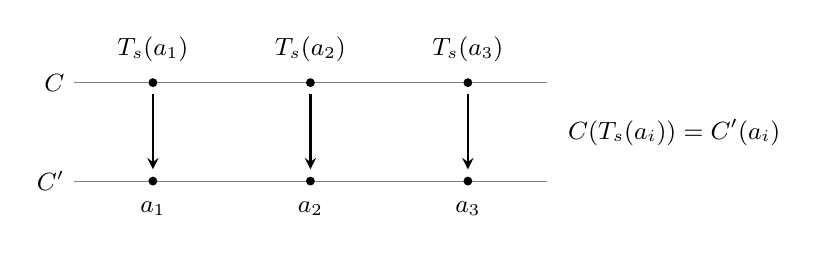
\begin{tikzpicture}[x=1cm,y=1cm,>=stealth, every node/.style={font=\small}]
 \draw[gray] (0,1.25) -- (6,1.25);
 \draw[gray] (0,0) -- (6,0);
 \node[anchor=east] at (0,1.25) {$C$};
 \node[anchor=east] at (0,0) {$C'$};
 \foreach \x/\i in {1/1,3/2,5/3} {
   \fill (\x,1.25) circle (1.6pt);
   \fill (\x,0) circle (1.6pt);
   \node[above=4pt] at (\x,1.25) {$T_s(a_{\i})$};
   \node[below=4pt] at (\x,0) {$a_{\i}$};
   \draw[->,thick] (\x,1.10) -- (\x,0.15);
 }
 \node[anchor=west] at (6.15,0.62) {$C(T_s(a_i))=C'(a_i)$};
\end{tikzpicture}

 \caption{On a matching transition from $C$ to $C'$, the points
 $a_i\in D_s$ and $T_s(a_i)$ receive the same coordinate rank:
 $C'(a_i)=C(T_s(a_i))$. Horizontal positions indicate the matched
 chart ranks schematically; their spacing carries no additional information.
 The diagram shows three points; the match
 is required on the whole finite domain $D_s$.}
 \label{fig:chart-transport}
\end{figure}
For one representative of each inverse pair, couple two charts with
law $\nu$ so that \eqref{eq:chart-match} holds with probability at least
$1-\epsilon$.
Such a coupling exists by \eqref{eq:subtuple-TV}. For two laws $\mu,\mu'$
on the same finite set, place mass $\min\{\mu(a),\mu'(a)\}$ at each
diagonal pair $(a,a)$ and couple the remaining masses arbitrarily.
The matching probability is $1-\TV(\mu,\mu')$.
Apply this to the laws of $C(T_s(D_s))$ and $C'(D_s)$, then sample the
full charts from their conditional distributions.
Denote the resulting coupling by $\lambda_s$.
For the inverse index set
\[
 \lambda_{s^{-1}}(C,C')=\lambda_s(C',C).
\]
This gives the inverse version of \eqref{eq:chart-match}, with the same
success probability.

Discard charts of zero $\nu$-mass and start $C_0$ with law $\nu$.
At each step choose a fresh uniform
letter $s\in\cS$, independently of the past. From the current chart $C$,
then choose $C'$ with probability $\lambda_s(C,C')/\nu(C)$ and record
$(C,s,C')$. The first marginal of $\lambda_s$ is $\nu$, so these
conditional probabilities sum to one.
Its stationary edge mass is
\begin{equation}\label{eq:chart-edge-mass}
 \frac{1}{|\cS|}\lambda_s(C,C'),
\end{equation}
which is invariant under $(C,s,C')^*=(C',s^{-1},C)$.
We have therefore constructed a finite stationary reversible marked
chain with independent uniform letters. At stationarity, each step
fails \eqref{eq:chart-match} with probability at most $\epsilon$.
\end{proof}

\section{Two levels from reduced words}\label{sec:action}

We construct a sum of periodic functions along a word of increasing
homeomorphisms. For a word with nonempty reduced form, this sum has one
value at integer points and another at the integer translates of the
image of $0$; the two values
differ by the reduced length of the word. These two interlaced families
will supply the alternating prefix sums in the walk construction.

Let $\cS=\{u,v,u^{-1},v^{-1}\}$, with positive letters $u,v$ and
negative letters $u^{-1},v^{-1}$.
A word is \emph{reduced} if it has no adjacent inverse letters.
Its reduced form is obtained by scanning from left to right: delete the
last retained letter when its inverse arrives, and append the new letter
otherwise.
Choose intervals $[\alpha_s,\beta_s]\subset(0,1)$, $s\in\cS$,
with positive lengths and pairwise disjoint closures, and put
\[
 \cA_s=\bigcup_{j\in\Z}[\alpha_s+j,\beta_s+j).
\]

\begin{lemma}\label{lem:action}
There are increasing homeomorphisms $h_s:\R\to\R$ such that
\begin{align}
 h_s(y+1)&=h_s(y)+1, & h_{s^{-1}}&=h_s^{-1},\label{eq:periodic-action}\\
 h_s(\R\setminus\cA_{s^{-1}})&=\cA_s,
 & |h_s(y)-y|&<2.\label{eq:pingpong}
\end{align}
For a word $w=s_1\cdots s_k$, write
$h_w=h_{s_1}\circ\cdots\circ h_{s_k}$, with $h_\varnothing$ the identity.
If $w$ is nonempty and reduced, then
\begin{equation}\label{eq:interior}
 h_w(0)\in\operatorname{int}(\cA_{s_1});
\end{equation}
in particular, $h_w(0)\notin\Z$.
\end{lemma}

\begin{proof}
For positive $s$, define $h_s$ to be affine on the intervals between
the following three points, with the indicated values:
\[
 \begin{array}{c|ccc}
 y&\alpha_{s^{-1}}&\beta_{s^{-1}}&\alpha_{s^{-1}}+1\\ \hline
 h_s(y)&\beta_s-1&\alpha_s&\beta_s.
 \end{array}
\]
Both slopes are positive. Extend by $h_s(y+1)=h_s(y)+1$, and define
$h_{s^{-1}}=h_s^{-1}$.
The complement intervals
$[\beta_{s^{-1}}+j,\alpha_{s^{-1}}+j+1)$ map exactly onto
$[\alpha_s+j,\beta_s+j)$, proving the set identity for positive letters.
Taking complements and inverses proves it for negative letters.
At the breakpoints $|h_s(y)-y|<2$; the difference is affine between
breakpoints and periodic. The same displacement bound holds for inverses.

The point $0$ lies outside all the arc closures. Reading a reduced word
from right to left, the first image lies in the interior of the arc of
the rightmost letter. At every subsequent step this arc is disjoint
from the inverse arc of the next letter, so the image enters the interior
of that letter's arc. This proves \eqref{eq:interior}.
\end{proof}

Subtracting one for negative letters makes the interval indicator change
sign under reversal. Define the periodic integer-valued functions
\begin{equation}\label{eq:chi}
 \chi_s(y)=\one_{\cA_s}(y)-\one_{\{s\text{ is negative}\}}.
\end{equation}
The complement identity gives
\[
 \one_{\cA_{s^{-1}}}(h_s^{-1}(y))=1-\one_{\cA_s}(y),
\]
and hence
\begin{equation}\label{eq:chi-cancellation}
 \chi_{s^{-1}}(h_s^{-1}(y))=-\chi_s(y).
\end{equation}
For a word $w=s_1\cdots s_k$ and an initial point $y_0=y$, set
\begin{equation}\label{eq:c-word}
 y_i=h_{s_i}^{-1}(y_{i-1}),\qquad
 c_w(y)=\sum_{i=1}^k\chi_{s_i}(y_{i-1}).
\end{equation}
The final point is $y_k=h_w^{-1}(y)$.
Periodicity of the $\chi_s$ and \eqref{eq:periodic-action} give
$c_w(y+1)=c_w(y)$.
Deleting adjacent inverse letters leaves both the final point and
$c_w(y)$ unchanged, by \eqref{eq:chi-cancellation}.

\begin{lemma}[Two levels]\label{lem:two-levels}
Let the reduced form of $w$ have length $\ell>0$, with $n_+$ positive
letters and $n_-$ negative letters. For every $j\in\Z$,
\begin{equation}\label{eq:two-levels}
 c_w(j)=-n_-,\qquad c_w(h_w(0)+j)=n_+.
\end{equation}
\end{lemma}

\begin{proof}
We may replace $w$ by its reduced form $t_1\cdots t_\ell$.
Start first at $j$. Before the first letter the point is outside every
arc. If the point before $t_i$ is outside $\cA_{t_i}$, its inverse
image under $h_{t_i}$ belongs to $\cA_{t_i^{-1}}$; this is disjoint
from $\cA_{t_{i+1}}$ because the word is reduced.
Thus every indicator $\one_{\cA_{t_i}}$ in \eqref{eq:c-word} is zero,
giving the first equality.

Starting instead at $h_w(0)+j$, the point before $t_i$ is
$h_{t_i\cdots t_\ell}(0)+j$. By \eqref{eq:interior} it lies in
$\cA_{t_i}$, so every indicator is one. The sum is $\ell-n_-=n_+$.
\end{proof}

For a word with nonempty reduced form, let $z\in(0,1)$ be the fractional
part of $h_w(0)$. By periodicity, the two levels occur at the interlaced
points
\[
 j<z+j<j+1,\qquad
 c_w(j)=-n_-,\quad c_w(z+j)=n_+\qquad(j\in\Z).
\]
The next construction places these points at fixed coordinate ranks
throughout a chart trajectory.

\section{Construction of the finite walks}\label{sec:walks}

We now combine chart transport with the two-level cocycle. On matching
transitions, moving landmarks keep their chart ranks; their prefix
values will then yield a norm lower bound. We finish by checking how
often matching transitions and a long reduced word occur together.

\begin{proof}[Proof of Proposition~\ref{prop:walks}]
Fix a norm $N$ as in the proposition. We first construct labels with a
common nonzero norm and normalize them at the end.
For $k\geq1$, put
\[
 D_k=N(\underbrace{1,-1,\ldots,1,-1}_{k\text{ pairs}}).
\]
These numbers are positive, and spreading invariance and the triangle
inequality give $D_{k+l}\leq D_k+D_l$.

\par\smallskip
\Needspace{5\baselineskip}
\noindent\emph{Step 1: the finite chart chain.}
Fix an integer $n\geq1$, and let
\[
 L=8(n+1),\qquad \epsilon=\frac1{10n}.
\]
Use the homeomorphisms of Lemma~\ref{lem:action}.
The landmarks below record the interval endpoints used by labels and
all orbit points needed to follow $n$ steps. The integer shifts provide
a margin around the label window. Let $\Lambda$ be the following finite
subset of $\R$, in its usual order:
\begin{equation}\label{eq:landmarks}
 \begin{split}
 \Lambda={}&\{\alpha_s+j,\beta_s+j:s\in\cS,\ 0\leq j<L\}\\
 &\quad\cup
 \{h_w(0)+j: |w|\leq n,\ -2n\leq j\leq L+2n\}.
 \end{split}
\end{equation}
All displayed shifts $j$ are integers, $|w|$ denotes the length before
reduction, the empty word is included, and coincident points are counted
only once.
For each $s$ use the partial order-preserving bijection
\[
 T_s=h_s|_{D_s},\qquad
 D_s=\{a\in\Lambda:h_s(a)\in\Lambda\}.
\]
Its inverse is $T_{s^{-1}}$.
Proposition~\ref{prop:chart-transport} gives a finite stationary
reversible marked chain on charts; denote its stationary chart law by
$\nu$.
Call a transition $(C,s,C')$ \emph{good} when
\begin{equation}\label{eq:good}
 C'(a)=C(h_s(a))\qquad(a\in D_s).
\end{equation}
Every step is good with probability at least $1-\epsilon$.

For positive $s$, define
\begin{equation}\label{eq:labels}
 g(C,s,C')=\sum_{j=0}^{L-1}
     \bigl(b_{C(\alpha_s+j)}-b_{C(\beta_s+j)}\bigr),
\end{equation}
and define negative labels by oddness:
$g(C,s,C')=-g(C',s^{-1},C)$.
Strict increase of the charts and spreading invariance imply
\begin{equation}\label{eq:one-step-norm}
 N(g(C,s,C'))=D_L
\end{equation}
for every transition, good or otherwise.

\par\smallskip
\Needspace{5\baselineskip}
\noindent\emph{Step 2: transport along a good trajectory.}
Consider a trajectory $(C_{i-1},s_i,C_i)_{i=1}^n$ all of whose steps
are good, and let $w=s_1\cdots s_n$ have reduced length $\ell>0$.
Put
\[
 m=\lfloor h_w(0)\rfloor,\qquad z=h_w(0)-m.
\]
Since every letter moves every point by less than $2$, $|h_w(0)|<2n$,
so $-2n\leq m\leq2n-1$; and \eqref{eq:interior} gives $0<z<1$.
For the integers $L/4\leq j\leq3L/4$, define
\begin{equation}\label{eq:rank-pairs}
 r_j=C_0(j),\qquad t_j=C_0(z+j).
\end{equation}
These points belong to $\Lambda$ by \eqref{eq:landmarks}, and
$r_j<t_j<r_{j+1}$ whenever the indices occur.

For either starting point $y_0=j$ or $y_0=z+j$, follow
$y_i=h_{s_i}^{-1}(y_{i-1})$.
For the first family,
\[
 y_i=h_{s_i^{-1}\cdots s_1^{-1}}(0)+j;
\]
for the second,
\[
 y_i=h_{s_{i+1}\cdots s_n}(0)+j-m.
\]
The words have length at most $n$, and the shifts lie in
$[-2n,L+2n]$. Thus all these points belong to $\Lambda$.
Moreover, for every $0\leq i\leq n$,
\begin{equation}\label{eq:transport-bounds}
 j-2n<y_i<j+1+2n,
\end{equation}
and the whole interval lies in $(0,L)$ for the chosen range of $j$.
Because $h_{s_i}(y_i)=y_{i-1}$, goodness gives
\begin{equation}\label{eq:transport-rank}
 C_i(y_i)=C_{i-1}(y_{i-1})=C_0(y_0).
\end{equation}

\par\smallskip
\Needspace{5\baselineskip}
\noindent\emph{Step 3: cumulative coefficient sums.}
Let
\[
 G=\sum_{i=1}^n g(C_{i-1},s_i,C_i),\qquad
 F(k)=\sum_{a=1}^k G_a\quad(0\leq k\leq B).
\]
Every label has total coefficient sum zero, so $F(0)=F(B)=0$.
For landmarks $\alpha<\beta$ and $y$, strict increase of a chart gives
\[
 \sum_{a\leq C(y)}(b_{C(\alpha)}-b_{C(\beta)})_a
 =\one_{[\alpha,\beta)}(y).
\]
This explains the half-open interval convention.
Evaluate $F$ at a transported rank $C_0(y_0)$.
For a positive step, \eqref{eq:labels}, \eqref{eq:transport-rank},
and $y_{i-1}\in(0,L)$ therefore give the contribution
$\one_{\cA_{s_i}}(y_{i-1})$.
For a negative step the label is read in chart $C_i$. Since $y_i\in(0,L)$
as well, its contribution is
\[
 -\one_{\cA_{s_i^{-1}}}(y_i)
 =\one_{\cA_{s_i}}(y_{i-1})-1.
\]
Thus in both cases the contribution is $\chi_{s_i}(y_{i-1})$, and
\begin{equation}\label{eq:F-cocycle}
 F(C_0(y_0))=c_w(y_0).
\end{equation}
Reduction is applied to this scalar expression; $G$ retains all $n$
original edge labels.
Let $n_+,n_-$ be the numbers of positive and negative letters in the
reduced word. Lemma~\ref{lem:two-levels}, applied with the integer shifts
$j$ and $j-m$, now gives
\begin{equation}\label{eq:F-levels}
 F(r_j)=V:=-n_-,\qquad F(t_j)=U:=n_+,
 \qquad U-V=\ell.
\end{equation}

\par\smallskip
\Needspace{5\baselineskip}
\noindent\emph{Step 4: converting oscillations to norm.}
Put $a=L/4$ and $b=3L/4$.
The selected cuts and their prefix sums determine every consecutive
block sum:
\[
\begin{array}{c|cccccccc}
 \text{cut}&0&r_a&t_a&r_{a+1}&\cdots&t_{b-1}&r_b&B\\
 F&0&V&U&V&\cdots&U&V&0\\
 \text{block sum}& &V&\ell&-\ell&\cdots&\ell&-\ell&-V
\end{array}
\]
The last row gives the sum of the block ending at that cut.
There are $b-a=L/2$ inner pairs. Replacing every block by its sum is
contractive and yields
\begin{equation}\label{eq:compressed}
 (V,\underbrace{\ell,-\ell,\ldots,\ell,-\ell}_{L/2\text{ pairs}},-V).
\end{equation}
The last block is nonempty, since the rank $t_b$ from
\eqref{eq:rank-pairs} satisfies $r_b<t_b\leq B$.
We control the endpoint contribution by combining the estimate from all
oscillations with the estimate from a single level.
Subtracting the endpoint array by the triangle inequality and using
$|V|\leq\ell$ gives
\[
 N(G)\geq\ell D_{L/2}-|V|D_1
       \geq\ell(D_{L/2}-D_1).
\]
Independently, partitioning just at an $r_j$ or a $t_j$ gives the arrays
$(V,-V)$ and $(U,-U)$. Hence
\[
 N(G)\geq\max\{|V|,U\}D_1\geq\frac\ell2D_1.
\]
For nonnegative $A,B$, $\max\{A-B,B/2\}\geq A/3$.
Together with $D_L\leq2D_{L/2}$, this proves
\begin{equation}\label{eq:linear-displacement}
 N(G)\geq\frac\ell3D_{L/2}\geq\frac\ell6D_L.
\end{equation}

\par\smallskip
\Needspace{5\baselineskip}
\noindent\emph{Step 5: probability and normalization.}
The probability that at least one transition fails to be good is at most
$n\epsilon=1/10$, by stationarity and the union bound.
Without conditioning on goodness, the letters are independent and
uniform in $\cS$.
As letters are appended, the reduced length has conditional expected
increment $1/2$ when positive, since exactly one of the four letters
cancels its last letter; at zero the increment is $1$.
Thus $\E\ell\geq n/2$. Since $0\leq\ell\leq n$,
\[
 \frac n2\leq\E\ell
 \leq\frac n4+n\Prob\{\ell\geq n/4\},
 \qquad\text{so}\qquad
 \Prob\{\ell\geq n/4\}\geq\frac14.
\]
With probability at least $1/4-1/10=3/20$, all steps are good and
$\ell\geq n/4$. On this event \eqref{eq:linear-displacement} gives
$N(G)\geq nD_L/24$. Every edge label has norm $D_L>0$ by
\eqref{eq:one-step-norm}, so dividing all labels by $D_L$ proves the
proposition.
\end{proof}

\appendix
\setcounter{equation}{0}
\renewcommand{\theequation}{\thesection.\arabic{equation}}
\section{Construction of the spreading norm}\label{app:norm}

We prove the ordered-norm lemma used in the reduction.
Its spreading-model and subdivision steps follow the approach of Brunel
and Sucheston \cite{BrunelSucheston1974,BrunelSucheston1975}; their later
work develops the resulting equal-sign-additive basis
\cite{BrunelSucheston}. The classical conclusion, recorded in
\cite[Theorem~2.2]{Ostrovskii}, is that every nonreflexive Banach space
finitely represents a Banach space with an equal-sign-additive basis.
We give the finite-array construction of the norm properties needed here.

\begin{proof}[Proof of Lemma~\ref{lem:ordered-norm}]
By \eqref{eq:superreflexive-characterization}, there is a nonreflexive
Banach space $Y$ finitely representable in $X$. Identify $Y$ with its
canonical image in $Y^{**}$, and choose
$v\in B_{Y^{**}}$ and $d>0$ with $\dist(v,Y)>d$.

The first limit will produce a spreading norm $N_0$, finitely representable
in $Y$, that controls coefficient prefix sums. A second limit averages
increasingly fine subdivisions. It preserves these properties and makes
the resulting norm $N$ invariant under subdivision. Same-sign merging
then preserves $N$, and convexity gives contractive merging for arbitrary
adjacent coefficients.

\par\smallskip
\Needspace{5\baselineskip}
\noindent\emph{Step 1: finite triangular arrays.}
For every integer $M\geq1$, we construct
$y_1,\ldots,y_M\in B_Y$ and $f_1,\ldots,f_M\in B_{Y^*}$ such that
\begin{equation}\label{eq:triangle}
 f_i(y_j)=0\quad(j<i),\qquad
 |f_i(y_j)-d|\leq M^{-1}\quad(j\geq i).
\end{equation}
Suppose $y_1,\ldots,y_{i-1}$ have been chosen and let
$E=\Span\{y_1,\ldots,y_{i-1}\}$. The restriction map
$Y^{**}\to(E^\perp)^*$ is a quotient map with kernel the canonical
copy of $E$: Hahn--Banach extends every bounded functional on
$E^\perp\subseteq Y^*$ to all of $Y^*$ with the same norm, while finite
dimensionality gives
$(E^\perp)^\perp=E$. Thus the quotient norm of $v+E$ equals the norm
of its restriction to $E^\perp$. Hence
\[
 \norm{v|_{E^\perp}}=\dist(v,E)\geq\dist(v,Y)>d.
\]
We may therefore choose $f_i\in B_{Y^*}\cap E^\perp$ with $v(f_i)=d$,
by changing a sign and rescaling if necessary.
The finite-dimensional form of Goldstine's theorem gives
$y_i\in B_Y$ with $|f_h(y_i)-v(f_h)|\leq M^{-1}$ for $1\leq h\leq i$.
Indeed, $(v(f_1),\ldots,v(f_i))$ belongs to the closure of
$\{(f_1(y),\ldots,f_i(y)):y\in B_Y\}$: otherwise a separating linear
functional would give $v(f)>\sup_{y\in B_Y}f(y)=\|f\|$ for some
$f\in\Span\{f_1,\ldots,f_i\}$, contradicting $\|v\|\leq1$.
This proves \eqref{eq:triangle} inductively.

Read the vectors in the reverse order. For any subtuple
$y_{i_1},\ldots,y_{i_m}$ with $i_1>\cdots>i_m$, the functional $f_{i_j}$
annihilates the terms after the $j$th and approximates $d$ on the first
$j$ terms. Consequently,
\begin{equation}\label{eq:finite-prefix}
 d\max_{1\leq j\leq m}\abs{\sum_{h=1}^j a_h}
 -\frac1M\sum_{h=1}^m|a_h|
 \leq\norm{\sum_{h=1}^m a_h y_{i_h}}
 \leq\sum_{h=1}^m|a_h|.
\end{equation}

\par\smallskip
\Needspace{5\baselineskip}
\noindent\emph{Step 2: a spreading limit.}
Fix $k$. For each $m\leq k$, choose a finite grid in $[-1,1]^m$
with mesh at most $k^{-2}$ in the maximum norm. Color every increasing
$m$-subtuple of the reversed array by the list of the norms of its
grid combinations, rounded into intervals of length $k^{-1}$.
The number of colors is finite and independent of $M$.
The finite Ramsey theorem, applied successively for $m=1,\ldots,k$,
shows that, for sufficiently large $M=M_k\geq k^3$, there is a tuple
$(x_1^{(k)},\ldots,x_k^{(k)})$ on which all these colorings are homogeneous.
At each arity, thin a previously homogeneous set; homogeneity from
earlier arities persists under this thinning.
For fixed $m\leq k$ and $a\in[-1,1]^m$, the norms of the combinations
with coefficients $a$ on any two increasing $m$-subtuples differ by at most
\[
 k^{-1}+2mk^{-2}\leq3k^{-1}.
\]
The additional error follows from the upper bound in
\eqref{eq:finite-prefix}.

Taking a diagonal subsequence over all finite rational coefficient
tuples, and then using the common $\ell_1$ Lipschitz bound, gives limits
\[
 N_0(a_1,\ldots,a_m)
 =\lim_{k\to\infty}\norm{\sum_{i=1}^m a_i x_i^{(k)}}.
\]
The limits are compatible with appending zeros. The vanishing
subtuple oscillations give \eqref{eq:spreading} for $N_0$.
Passing to the limit in \eqref{eq:finite-prefix} yields
\begin{equation}\label{eq:N0-bounds}
 d\max_j\abs{\sum_{i=1}^j a_i}\leq N_0(a)\leq\sum_i|a_i|.
\end{equation}
The norm axioms pass to the limit, and the lower bound gives positive
definiteness. On each fixed coefficient cube the convergence is uniform,
by the common Lipschitz bound and compactness.
Moreover,
\begin{equation}\label{eq:nondegenerate}
 N_0(a)\geq\frac d2\max_i|a_i|,
\end{equation}
since every coefficient is the difference of two successive prefix sums.
Thus the maps $a\mapsto\sum_i a_i x_i^{(k)}$ give linear embeddings
of every fixed coordinate span into $Y$ with distortions tending to $1$.

\par\smallskip
\Needspace{5\baselineskip}
\noindent\emph{Step 3: averaging subdivisions.}
For positive integers $J_1,\ldots,J_m$, let $F_{\boldsymbol J}a$ be the
array obtained by replacing $a_i$ by $J_i$ copies of $a_i/J_i$.
Write $F_J$ when all multiplicities equal $J$.
If $J_i\leq M_i$ for every $i$, then
\begin{equation}\label{eq:dilation-monotone}
 N_0(F_{\boldsymbol M}a)\leq N_0(F_{\boldsymbol J}a).
\end{equation}
Indeed, in the $i$th block of length $M_i$, select a uniformly random
$J_i$-element subset and place $a_i/J_i$ in those positions, with zeros
elsewhere. Every resulting array is obtained from
$F_{\boldsymbol J}a$ by inserting zeros, so has the same $N_0$ norm.
Its mean is $F_{\boldsymbol M}a$, and convexity proves the claim.

It follows that
\begin{equation}\label{eq:N-definition}
 N(a)=\lim_{J\to\infty}N_0(F_Ja)
\end{equation}
exists. The bounds in \eqref{eq:N0-bounds} survive subdivision, because
the original prefix sums still occur at the ends of the blocks.
Consequently, for every $a=(a_1,\ldots,a_m)$,
\begin{equation}\label{eq:prefix-bounds}
 d\max_{1\leq j\leq m}\abs{\sum_{i=1}^j a_i}
 \leq N(a)\leq\sum_{i=1}^m|a_i|.
\end{equation}
Spreading invariance and the norm axioms also pass to the limit.
The functions $a\mapsto N_0(F_Ja)$ again have the common $\ell_1$
Lipschitz bound, so convergence is uniform on every fixed coefficient
cube. The lower bound \eqref{eq:nondegenerate} also holds for $N$.
Fix a source dimension $m$ and $\eta>0$. First choose $J$ so that $F_J$
embeds the $m$-dimensional $N$ span into the $mJ$-dimensional $N_0$ span
with distortion less than $1+\eta$.
Indeed, uniform additive convergence on the compact $N$-unit sphere,
together with \eqref{eq:nondegenerate}, gives uniform relative error.
Approximate this now fixed $N_0$ span in $Y$ with distortion less than
$1+\eta$, and then embed its finite-dimensional image into $X$ with
distortion less than $1+\eta$. The composite distortion is less than
$(1+\eta)^3$; letting $\eta\downarrow0$ proves \textup{(iii)}.

\par\smallskip
\Needspace{5\baselineskip}
\noindent\emph{Step 4: consecutive summation.}
First, $N$ is unchanged by every fixed varying-multiplicity subdivision:
\begin{equation}\label{eq:subdivision-invariance}
 N(F_{\boldsymbol J}a)=N(a).
\end{equation}
To see this, put $J_- =\min_iJ_i$ and $J_+=\max_iJ_i$.
The composite $F_rF_{\boldsymbol J}$ replaces each $a_i$ by $rJ_i$
equal pieces. Thus, for every $r$,
\[
 N_0(F_{rJ_+}a)
 \leq N_0(F_rF_{\boldsymbol J}a)
 \leq N_0(F_{rJ_-}a)
\]
by \eqref{eq:dilation-monotone}; let $r\to\infty$.

If adjacent nonzero coefficients have the same sign and rational ratio,
subdivide them into equal pieces. Subdividing their sum into the combined
number of pieces gives the identical array. Equation
\eqref{eq:subdivision-invariance} shows that merging these coefficients
preserves $N$. Continuity extends this statement to every same-sign
pair, and spreading invariance handles zeros.

Fix all other coefficients and fix $s\ne0$. The function
\[
 t\longmapsto N(\ldots,t,s-t,\ldots)
\]
is convex and is constant, at the merged norm $N(\ldots,s,\ldots)$,
on the nondegenerate interval with endpoints $0$ and $s$.
A convex function constant on a nondegenerate interval is at least that
constant everywhere: a smaller exterior value, together with the farther
endpoint, would force the nearer endpoint below that constant.
This proves \eqref{eq:merge} when $s\ne0$.
Letting $s\to0$ proves it for $s=0$ as well.
\end{proof}

\clearpage
\pdfbookmark[1]{References}{references}
\begin{thebibliography}{99}

\bibitem{Ball}
K.~Ball,
\emph{Markov chains, Riesz transforms and Lipschitz maps},
Geometric and Functional Analysis \textbf{2} (1992), 137--172.
\href{https://doi.org/10.1007/BF01896971}{doi:10.1007/BF01896971}.

\bibitem{Bourgain}
J.~Bourgain,
\emph{The metrical interpretation of superreflexivity in Banach spaces},
Israel Journal of Mathematics \textbf{56} (1986), 222--230.
\href{https://doi.org/10.1007/BF02766125}{doi:10.1007/BF02766125}.

\bibitem{BrunelSucheston1974}
A.~Brunel and L.~Sucheston,
\emph{On B-convex Banach spaces},
Mathematical Systems Theory \textbf{7} (1973), 294--299.
\href{https://doi.org/10.1007/BF01795947}{doi:10.1007/BF01795947}.

\bibitem{BrunelSucheston1975}
A.~Brunel and L.~Sucheston,
\emph{On J-convexity and some ergodic super-properties of Banach spaces},
Transactions of the American Mathematical Society \textbf{204} (1975), 79--90.
\href{https://doi.org/10.1090/S0002-9947-1975-0380361-2}{doi:10.1090/S0002-9947-1975-0380361-2}.

\bibitem{BrunelSucheston}
A.~Brunel and L.~Sucheston,
\emph{Equal signs additive sequences in Banach spaces},
Journal of Functional Analysis \textbf{21} (1976), 286--304.
\href{https://doi.org/10.1016/0022-1236(76)90041-0}{doi:10.1016/0022-1236(76)90041-0}.

\bibitem{Enflo}
P.~Enflo,
\emph{Banach spaces which can be given an equivalent uniformly convex norm},
Israel Journal of Mathematics \textbf{13} (1972), 281--288.
\href{https://doi.org/10.1007/BF02762802}{doi:10.1007/BF02762802}.

\bibitem{James}
R.~C.~James,
\emph{Super-reflexive Banach spaces},
Canadian Journal of Mathematics \textbf{24} (1972), 896--904.
\href{https://doi.org/10.4153/CJM-1972-089-7}{doi:10.4153/CJM-1972-089-7}.

\bibitem{JamesType2}
R.~C.~James,
\emph{Nonreflexive spaces of type 2},
Israel Journal of Mathematics \textbf{30} (1978), 1--13.
\href{https://doi.org/10.1007/BF02760825}{doi:10.1007/BF02760825}.

\bibitem{JohnsonSchechtman}
W.~B.~Johnson and G.~Schechtman,
\emph{Diamond graphs and super-reflexivity},
Journal of Topology and Analysis \textbf{1} (2009), 177--189.
\href{https://doi.org/10.1142/S1793525309000114}{doi:10.1142/S1793525309000114}.

\bibitem{LeeNaorPeres}
J.~R.~Lee, A.~Naor, and Y.~Peres,
\emph{Trees and Markov convexity},
Geometric and Functional Analysis \textbf{18} (2009), 1609--1659.
\href{https://doi.org/10.1007/s00039-008-0689-0}{doi:10.1007/s00039-008-0689-0}.

\bibitem{MendelNaor}
M.~Mendel and A.~Naor,
\emph{Markov convexity and local rigidity of distorted metrics},
Journal of the European Mathematical Society \textbf{15} (2013), 287--337.
\href{https://doi.org/10.4171/JEMS/362}{doi:10.4171/JEMS/362}.

\bibitem{Naor}
A.~Naor,
\emph{An introduction to the Ribe program},
Japanese Journal of Mathematics \textbf{7} (2012), 167--233.
\href{https://doi.org/10.1007/s11537-012-1222-7}{doi:10.1007/s11537-012-1222-7}.

\bibitem{NPSS}
A.~Naor, Y.~Peres, O.~Schramm, and S.~Sheffield,
\emph{Markov chains in smooth Banach spaces and Gromov-hyperbolic metric spaces},
Duke Mathematical Journal \textbf{134} (2006), 165--197.
\href{https://doi.org/10.1215/S0012-7094-06-13415-4}{doi:10.1215/S0012-7094-06-13415-4}.

\bibitem{Ostrovskii}
M.~I.~Ostrovskii,
\emph{Connections between metric characterizations of superreflexivity and the Radon--Nikodym property for dual Banach spaces},
Canadian Mathematical Bulletin \textbf{58} (2015), 150--157.
\href{https://doi.org/10.4153/CMB-2014-049-9}{doi:10.4153/CMB-2014-049-9}.

\bibitem{OstrovskiiRandrianantoanina}
M.~I.~Ostrovskii and B.~Randrianantoanina,
\emph{A new approach to low-distortion embeddings of finite metric spaces into non-superreflexive Banach spaces},
Journal of Functional Analysis \textbf{273} (2017), 598--651.
\href{https://doi.org/10.1016/j.jfa.2017.03.017}{doi:10.1016/j.jfa.2017.03.017}.

\bibitem{Pisier}
G.~Pisier,
\emph{Martingales with values in uniformly convex spaces},
Israel Journal of Mathematics \textbf{20} (1975), 326--350.
\href{https://doi.org/10.1007/BF02760337}{doi:10.1007/BF02760337}.

\end{thebibliography}

\end{document}
